\section{METHODOLOGY}\label{sec:methodology}
To create a valid throwing trajectory for a high-DOF, high-gain, position controlled robot, a desired line in $R^3$ in the direction of the desired velocity must be created.  Each point in the line is temporally separated by the robot's command period $T_r$.  All points in this line must be reachable.  Each point in the line must have poses that do not create a self-collision.  A valid throwing trajectory is created when the latter criteria are met.

\subsection{Self-Collision Detection}\label{sec:selfCollision}
Self-collision is an important when dealing with a high DOF robot.  Unwanted self-collisions can cause permanent damage to the physical and electrical hardware as well as causing the robot not to complete the given task.

To aid in the detection of self-collisions a detailed model of the Hubo KHR-4 was made in the widely used open-source robot simulation environment OpenRAVE\cite{diankovThesis}.  The model was created by exporting the three dimensional schematics that the physical robot was created with, to a format that OpenRAVE can use.  This was done in order to ensure an accurate and detailed model.  For these experiments we needed the external boundaries only; the internal geometry was replaced with a simplistic representation.  The external shell is the only part now visible, see Fig~\ref{fig:vHuboSparse} (Center).  The Proximity Query Package (PQP) was used to detect collisions between any two pieces of the robot's external shell.  Due to the high polygon count of the external shell the computation time of detecting a collision was on the magnitude of seconds.  It is advantageous to reduce this time if the system is to run live on the robot.  Computation time is decreased significantly when boundary/collision geometries are simplified due to the lower polygon count.  The collision geometries were further simplified to decrease computation time by making them primitives such as spheres, cylinder and boxes, see Fig~\ref{fig:vHuboSparse} (Right). 

%\begin{figure}[thpb]
%  \centering
%%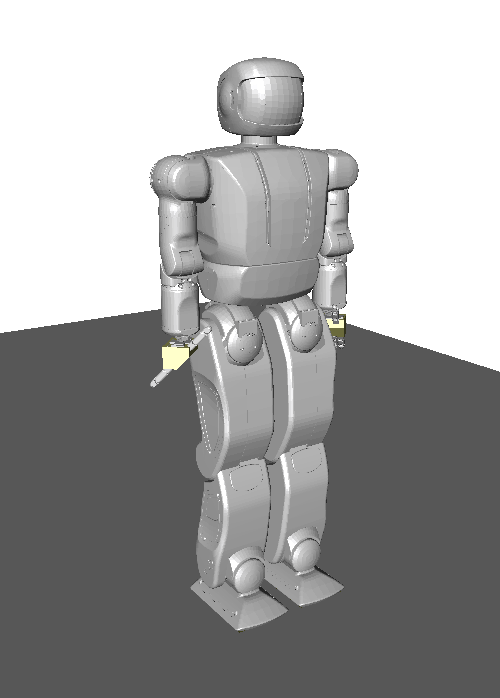
\includegraphics[width=0.5\columnwidth]{./pictures/hubo1s.png}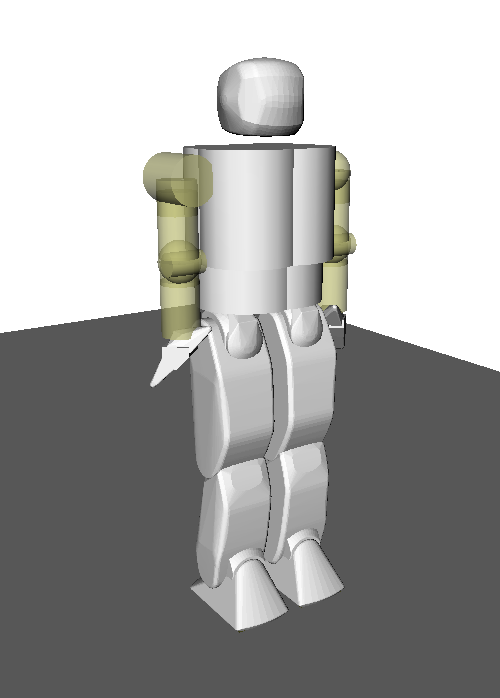
\includegraphics[width=0.5\columnwidth]{./pictures/hubo2s.png}
%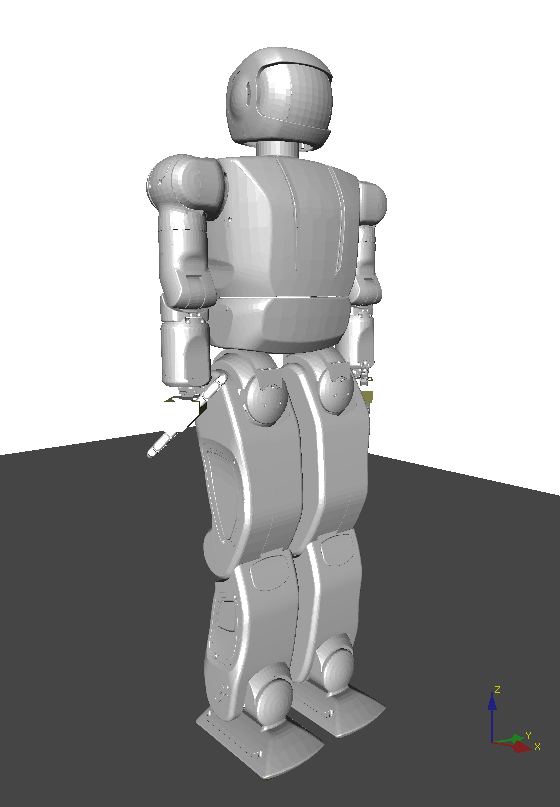
\includegraphics[width=0.5\columnwidth]{./pictures/final/hBody.png}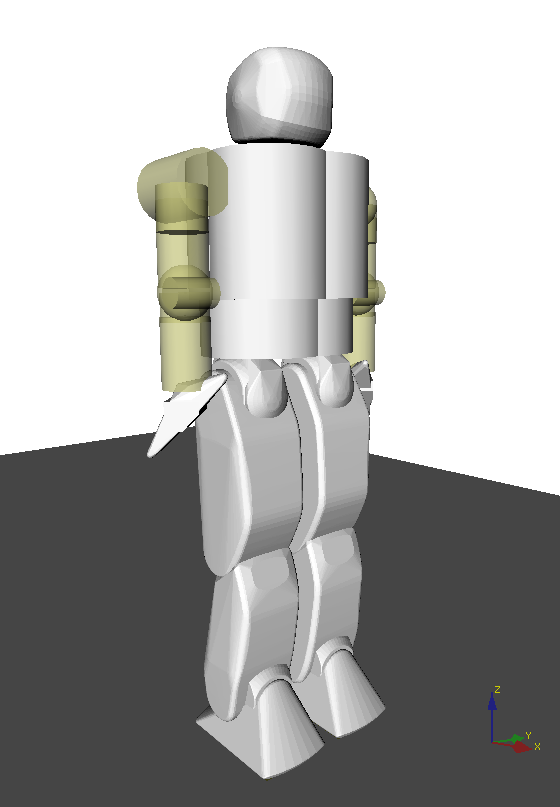
\includegraphics[width=0.5\columnwidth]{./pictures/final/hCol.png}
%  \caption{OpenRAVE model of Hubo KHR-4. Left: Model with protective shells.  Right: Collision Geometry  }
%  \label{fig:vHubo}
%\end{figure}

Joint limitations are added to the model to mimic the physical robot.  The model can be commanded the same configurations as the physical robot.  A pose is commanded to the model, PQP searches for any collisions.  With the simplified collision geometry self-collisions are detected on the order of milliseconds.  If there are no collisions then the pose can be applied to the physical robot.  A 5\% increase in volume between the simplified collision geometry and the high polygon geometry was added to ensure all of the physical robot's movements will not collide due to minor calibration errors.


\subsection{Reachable Area}\label{sec:rarea}
The desired end-effector velocity must be achieved with all joint limits and self-collision constraints satisfied at all times. Typical methods of determining reachability is to move each joint through its full range of motion for each DOF\cite{100034,springerlink:101007}. Due to the high DOF of the Hubo KHR-4 this method is not desirable.  A sampling method described in this work is similar to Geraerts et al.\cite{1570152}.  It was used to accommodate the high DOF system.

Both active and static joints must be defined to calculate the reachable area of a manipulator at a discrete time $N$.  The static joints are assumed to hold a fixed position at time step $N$.  Active joints are free to move to any position as long as it satisfies the joint angle limitations and does not create a self-collision.  A uniform random number generator is used to assign each active joint with an angle in joint space.  Each random angle assigned is within the valid range of motion of the respective joint.  The self-collision model described in Section~\ref{sec:selfCollision} is used to determine the self-collision status with the randomly assigned joint angles.  If there is no self-collision the end-effector position and transformation matrix $T$ are calculated using forward kinematics.

\begin{equation}\label{eq:fk1}
\mathbf{
\chi_i = \begin{bmatrix} R_{i} & \Gamma_{i} \\ 0 & 1 \end{bmatrix}
}
\end{equation}

\begin{equation}\label{eq:fk2}
T = \left[\chi_1 \cdot \chi_2 \cdot ... \cdot \chi_n \right]
\end{equation}
%\chi = \begin{bmatrix} R & \left[ \begin{array}{c} x \\ y \\ z \right]\end{array} \\ \left[ \begin{array}{cc} 0 & 0 & 0 & 1 \end{array} \right]  \end{bmatrix} 
%\chi = \begin{bmatrix} xz & xw \\ yz & yw \end{bmatrix} = \left[ \begin{array}{c} x \\ y \end{array} \right] \times \left[ \begin{array}{cc} z & w \end{array} \right] 
%\chi = \begin{bmatrix} R & T \\ 0 & 1 \end{bmatrix}
where $\chi_i$ is the transformation between joint $i-1$ and $i$, $R_i$ is the rotation of joint $i$ with respect to joint $i-1$ and $\Gamma_i$ is the translation of joint $i$ with respect to joint $i-1$, and $n$ is the number of joints in the kinematic chain.

The end-effector position and the joint angles used are recorded.  This process is repeated multiple times to form a sparse representation of reachable end-effector positions in $R^3$ and the corresponding joint angles in joint space.  The resulting representation is called the Sparse Reachable Map (SRM).  Fig.~\ref{fig:sparseRegion} shows a cross section of the SRM about the right shoulder between -0.40 $m$ to 0.40 $m$ on X, -0.40 $m$ to 0.40 $m$ on Z, and -0.21 to -0.22 $m$ on Y.  The blue points show valid end-effector locations with known kinematic solution in joint space.  Fig.~\ref{fig:vHuboSparse} shows the SRM of the entire right arm.  The SRM is used to calculate valid movement trajectories.


\begin{figure}[thpb]
  \centering
%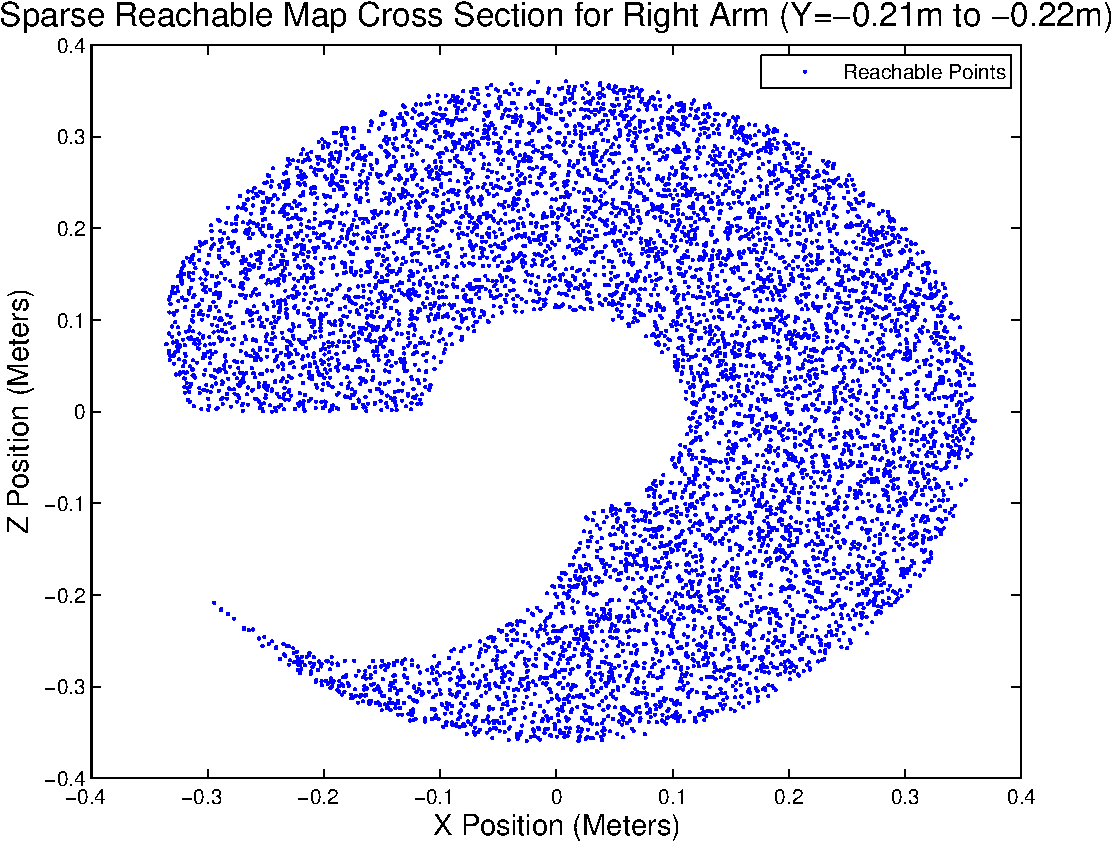
\includegraphics[width=1.0\columnwidth]{./MATLAB/reachable2DofR4p8.pdf}
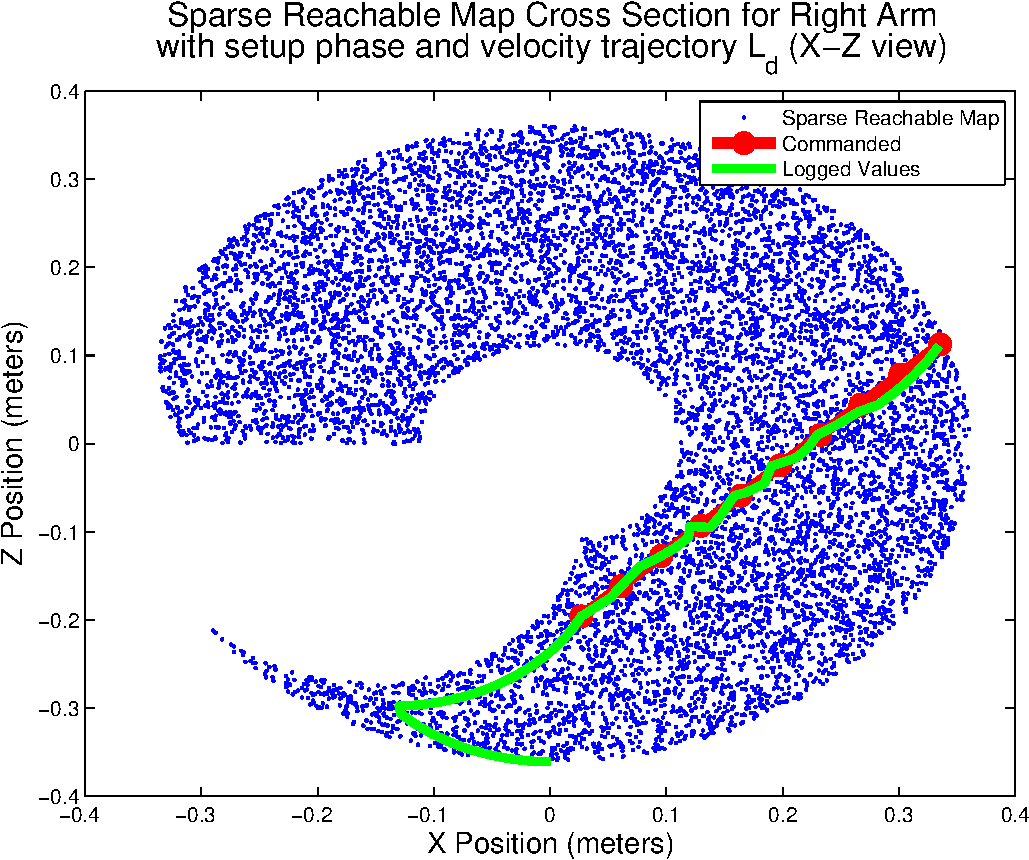
\includegraphics[width=1.0\columnwidth]{./MATLAB/throwTrajAct.pdf}
\caption{Cross section of the SRM about the right shoulder between -0.40 $m$ to 0.40 $m$ on X, -0.40 $m$ to 0.40 $m$ on Z, and -0.21 to -0.22 $m$ on Y.  (Blue) show valid end-effector locations with known kinematic solution in joint space. (Red) Commanded right arm end-effector position in $R^3$.  (Green) The logged joint space values converted to $R^3$ using forward kinematics.
}
  %\caption{Sparse region of reachable locations for the robot's right arm between -0.40m and 0.40m on X, -0.40m and 0.40m on Z, and -0.21 to -0.22m on Y.  Region created by randomly sampling from joint space.  (Blue) Points with valid kinematic solutions that do not cause a self-collision.  (Red) Commanded right arm end-effector position in $R^3$.  (Green) The logged joint space values converted to $R^3$ using forward kinematics.}
  \label{fig:sparseRegion}
\end{figure}

\begin{figure}[thpb]
  \centering
%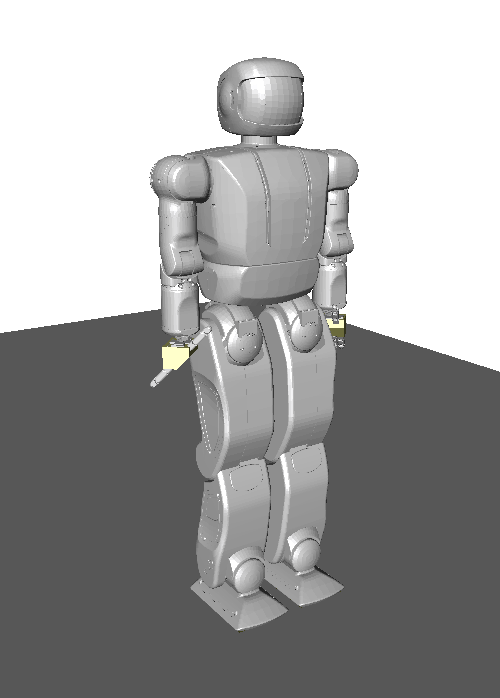
\includegraphics[width=0.5\columnwidth]{./pictures/hubo1s.png}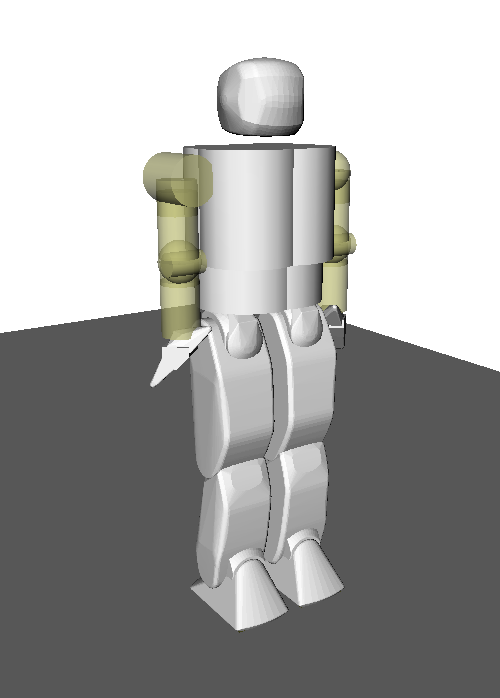
\includegraphics[width=0.5\columnwidth]{./pictures/hubo2s.png}
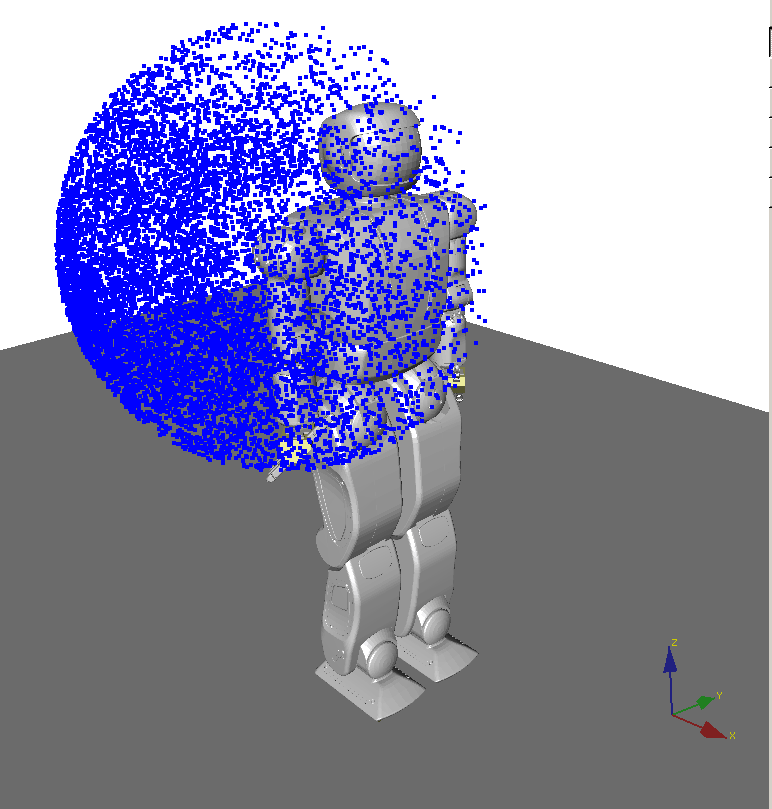
\includegraphics[width=0.36\columnwidth]{./pictures/final/SRM.png}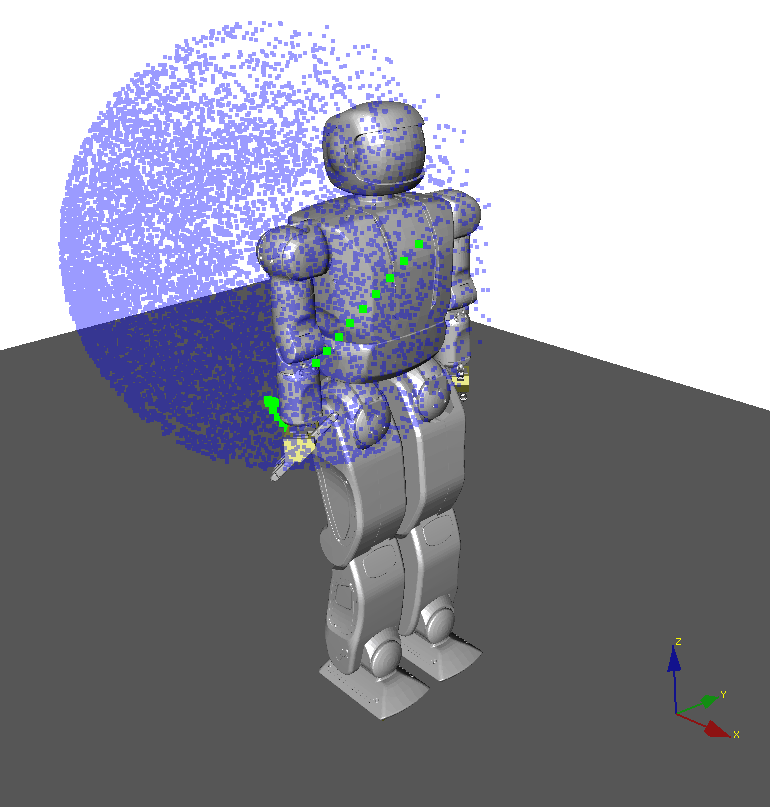
\includegraphics[width=0.36\columnwidth]{./pictures/final/ThrowTrajDiag.png}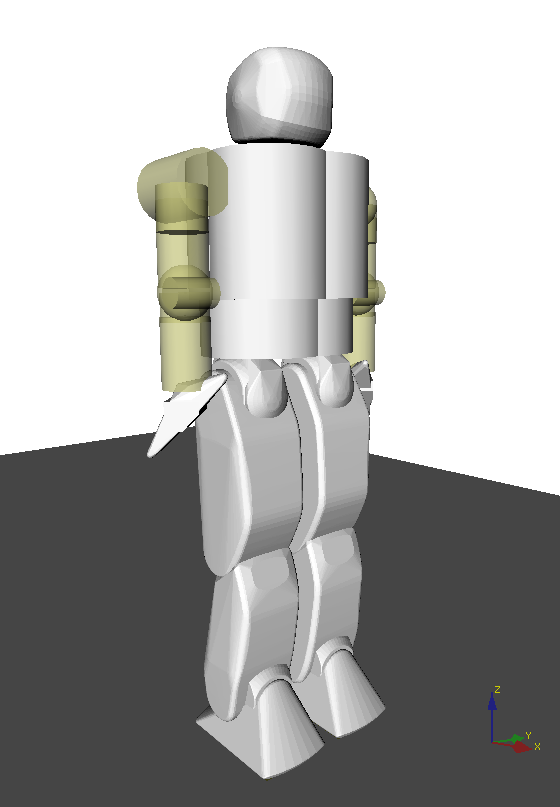
\includegraphics[width=0.28\columnwidth]{./pictures/final/hCol.png}
  \caption{OpenRAVE model of Hubo KHR-4. Left: Model with SRM of right arm.  Center: SRM (blue) with setup and velocity phase trajectories (green) Right: Collision Geometry  }
  \label{fig:vHuboSparse}
\end{figure}



\subsection{Trajectory Generation}\label{sec:trajGen}
An end-effector velocity, $\vec{V}_e$, is chosen based on target location, the well known equations of projectile motion, and the required velocity duration $t_e$.  $\vec{V}_e$ must be held for a time span of $t_e$. The release point must be within the time span $t_e$.  The magnitude of the velocity in the direction of $V_e$ immediately preceding time span $t_e$ must be less than or equal to the magnitude of $\vec{V}_e$ during $t_e$.  $t_e$ must be an integer multiple of the robot's actuator command period $T_r$.

A line $l_d$ in $R^3$ that passes through $(X_0, Y_0, Z_0)$ in the direction of $\vec{V}_e$ is created.  $\vec{L}_d$ is the discrete representation of $l_d$.  Each point in $\vec{L}_d$, $(X_0, Y_0, Z_0)$, $(X_1, Y_1, Z_1)$ $\cdots$ $(X_n, Y_n, Z_n)$, are separated by a time span $T_r$.

%A line, $L_d$, in $R^3$ is created with the origin $(x_0, y_0, z_0)$ in the direction of \vec{$V_e$}.  Each subsequent point in the line $(X_1, Y_1, Z_1)$, $(X_2, Y_2, Z_2)$ $\cdots$ $(X_n, Y_n, Z_n)$ are separated by a time span $T_r$.

The desired velocity is defined as

\begin{equation}
\vec{V}_d = [V_x\hat{i}, V_y\hat{j}, V_z\hat{k}]
\end{equation}

%\begin{equation}
%|V_e| =  \sqrt{V_x^2i+V_y^2+j+V_z^2k}
%\end{equation}

%\begin{equation}
%|L_d(N)_n^{n+1}| = \frac{\sqrt{\Delta X^2i + \Delta Y^2j + \Delta Z^2k}}{T_r}
%\end{equation}

%\begin{equation}
%\Delta L_d(N)_n^{n+1} = \frac{\Delta Xi + \Delta Yj + \Delta Zk}{T_r}
%\end{equation}

The line $\vec{L}_d(n)$ is defined as

\begin{equation}
\vec{L}_d(n) = [X_n\hat{i}, Y_n\hat{j} , Z_n\hat{k}]
\end{equation}

where $n$ is the current zero based time step index value for the time span $t_e$.  The change in $\vec{L}_d$ between time step $0$ and $n$ must be equal to our desired velocity $\vec{V}_d$.

%\begin{equation}
%\Delta L_d(N)_n^{n+1} = \Delta Xi + \Delta Yj + \Delta Zk
%\end{equation}

\begin{equation}
\frac{\Delta \vec{L}_d|_{0}^{n}}{n \cdot T_r} = \vec{V}_d
\end{equation}

%\begin{equation}
%V_di+V_dj+V_dk = \frac{\Delta Xi + \Delta Yj + \Delta Zk}{T_r}
%\end{equation}

%\begin{equation}
%V_d = \frac{[\Delta Xi, \Delta Yj, \Delta Zk]}{T_r}\Bigr\rvert_{n-1}^{n}
%\end{equation}

%Break up into its $i$, $j$, and $k$ components.
thus
\begin{equation}
\vec{V}_d = \frac{\vec{L}_d(n) - \vec{L}_d(0)}{n \cdot T_r}
\end{equation}

%\begin{eqnarray} 
%V_di & = &  \frac{\Delta Xi}{T_r}  =  \frac{X_{n+1} - X_n}{T_r}\\
%V_dj & = &  \frac{\Delta Yi}{T_r}  =  \frac{Y_{n+1} - Y_n}{T_r}\\
%V_dk & = &  \frac{\Delta Zi}{T_r}  =  \frac{Z_{n+1} - Z_n}{T_r}
%\end{eqnarray}
The line $\vec{L}_d$ at time step $n$ can now be defined in terms of $\vec{V}_d$, $T_r$, the origin $\vec{L}_d(0)$, and the current zero based time step index value $n$.

\begin{equation}
\vec{L}_d(n) = n \cdot T_r \cdot \vec{V}_d + \vec{L}_d(0)
\end{equation}


%Solve for the current step $n$ in terms of the origin $(X_0, Y_0, Z_0)$

%\begin{eqnarray} 
%X_n & = & n(V_di \cdot T_r) + X_0  \\
%Y_n & = & n(V_dj \cdot T_r) + Y_0  \\
%Z_n & = & n(V_dk \cdot T_r) + Z_0  
%\end{eqnarray}

%The line $L_d$ can now be defined in terms of the origin $(X_0, Y_0, Z_0)$ and the current zero based time step index value $n$.

%\begin{equation}
%L_d(n) = n \cdot V_d \cdot T_r + L_d(0)
%\end{equation}


where 

\begin{equation}
\vec{L}_d(0) = \left[X_0, Y_0, Z_0\right]
\end{equation}

%\begin{eqnarray} 
%L_d(n) 	&	= &	(n \cdot V_x \cdot T_r + X_0)i   \\  
%				&	  & + (n \cdot Y_x \cdot T_r + Y_0)j   \\
%				&   & + (n \cdot Z_x \cdot T_r + Z_0)k
%\end{eqnarray}

%\begin{equation} 
%L_d(n) 		= 	(n \cdot V_di \cdot T_r + X_0)i    
%				 + (n \cdot V_dj \cdot T_r + Y_0)j   	
%				 + (n \cdot V_dk \cdot T_r + Z_0)k
%\end{equation}

The line $\vec{L}_d$ is the trajectory the robot's end-effector must follow during the time span $t_e$.  The starting point $\vec{L}_d(0)$ must be found so that $\vec{L}_d$ is within the reachable area.  $\vec{L}_d(0)$ is set to a random starting points chosen within the SRM.  

\begin{equation}
\vec{L}_d(0) \in SRM
\end{equation}

All subsequent points in $\vec{L}_d$ must fall within some Euclidean distance $d$ from any point in SRM.  If one of the points in $\vec{L}_d$ fails this criteria a new random point is chosen for $\vec{L}_d(0)$ and the process is repeated. 

Once an $\vec{L}_d$ is found that fits the above criteria the inverse kinematic solution must be found for each point and checked for reachability.  Smaller values of $d$ will increase the probability $\vec{L}_d$ is within the reachable area defined in the SRM however more iterations will be required to find a valid $\vec{L}_d$.  Larger values of $d$ will decrease the number of iterations needed to find a valid $\vec{L}_d$ however the probability of $\vec{L}_d$ being in the reachable area is decreased.  In addition larger values of $d$ decreases the system's ability to properly map near sharp edges in the SRM.  Increasing the number of samples in the SRM will allow for larger values for $d$.

\subsection{Inverse Kinematics}\label{sec:ik}
The trajectory $\vec{L}_d$ has one point with a known kinematic solution in $R^3$ and in joint space, $\vec{L}_d(0)$.  The joint space kinematic solutions for points $\vec{L}_d(1) \rightarrow \vec{L}_d(n)$ are unknown.  Mapping the robot's configuration $\vec{q} \in Q$ to the desired end-effector goal $\vec{x}_g \in X$, where $Q$ is the robot's configuration space and $X$ is in $R^3$, is done using Jacobian Transpose Controller used by Weghe et al.\cite{4813913}.  Weghe shows the Jacobian as a linear map from the tangent space of $Q$ to $X$ and is expressed as

\begin{equation}
\dot{\vec{x}} = J\dot{\vec{q}}
\end{equation}

  The Jacobian Transpose method is used because of the high DOF of the Hubo KHR-4.  Under the assumption of an obstacle-free environment the Jacobian Transpose Controller is guaranteed to reach the goal.  A proof is shown by Wolovich et al.\cite{4048118}.

To drive the manipulator from its current position $x$ to the goal positions $x_g$ the error $e$ is computed and the control law is formed.

\begin{equation}
\vec{e} = \vec{x}_g - \vec{x}
\end{equation}

\begin{equation}
\dot{\vec{q}} = kJ^T\vec{e}
\end{equation}

where k is a positive gain and self-collisions are ignored.  The instantaneous motion of the end-effector is given by

\begin{equation}
\dot{\vec{x}} = J\dot{\vec{q}} = J(kJ^T\vec{e})
\end{equation}

The final pose $\vec{q}$ for our goal position $\vec{x}_g$ can now be found.

The Jacobian Transpose method works best when there is a small difference between the current position $\vec{x}$ and the goal position $\vec{x_g}$.  $\vec{L}_d(0)$ is known both in $X$ and in $Q$ and is the starting point.

\begin{equation}
\vec{x} = \vec{L}_d(0)
\end{equation}

\begin{equation}
\vec{q}_0 = SRM  \left( \vec{L}_d(0) \right)
\end{equation}

The goal position $\vec{x}_g$ is set to the next point in $\vec{L}_d$

\begin{equation}
\vec{x}_g = \vec{L}_d(1)
\end{equation}

The pose $\vec{q}_1$ can now be calculated

\begin{equation}
\vec{q}_1 = \vec{q}_0 + \dot{\vec{q}}_0 = \vec{q}_0 + kJ^T\vec{e}|_{\vec{x}}^{\vec{x}_g}
\end{equation}

where $\vec{x}_g = \vec{L}_d(0)$ and $\vec{x} = \vec{L}_d(1)$.  $\vec{L}_d(1)$ is now known both in $X$ and in $Q$.  Now $\vec{x} = \vec{L}_d(1)$ and the process is repeated until all points in $L_d$ are known both in $X$ and $Q$.




%\begin{figure}[thpb]
%  \centering
%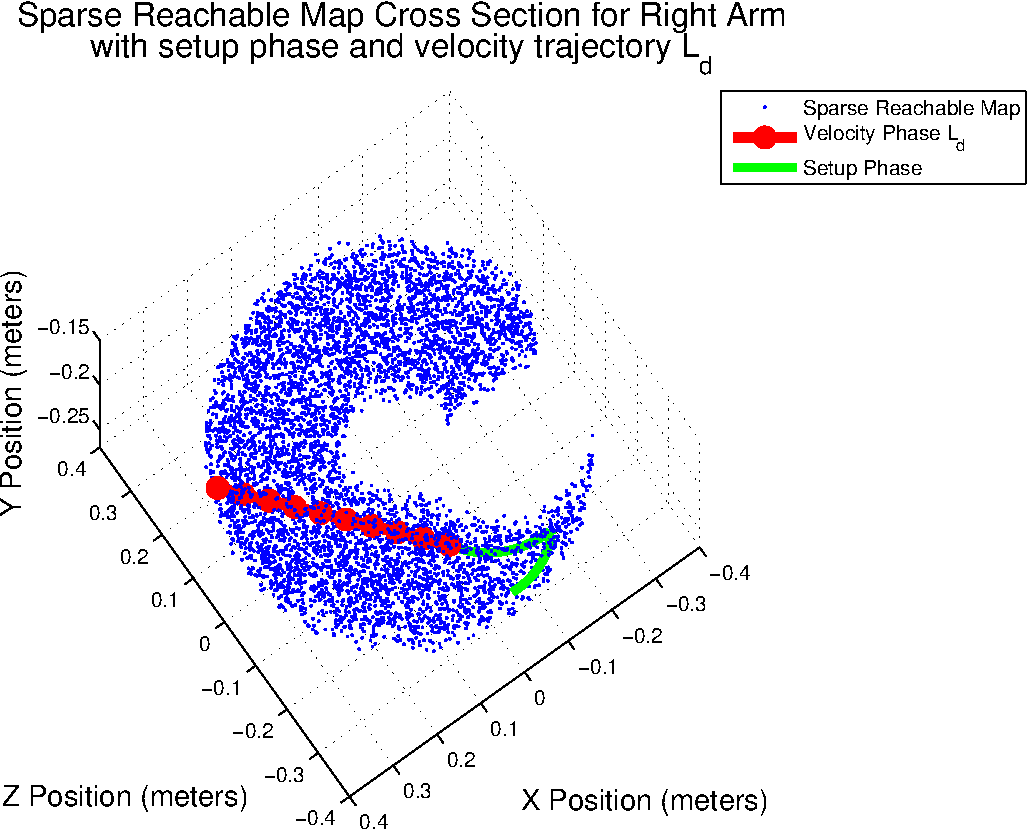
\includegraphics[width=1.0\columnwidth]{./MATLAB/throwTraj3D.pdf}
%  \caption{Sparse Reachable Map Cross Section for Right Arm with setup phase and velocity trajectory $L_d$ }
%  \label{fig:3dThrowPlot1}
%\end{figure}

\subsection{On-Line Trapezoidal Motion Profile}\label{sec:trap}

The robot's starting position $\vec{x}_0$ is not guaranteed to be the same as the
first point in the velocity trajectory $\vec{L}_d$.  To avoid over large
accelerations when giving this step input from $\vec{x}_0$ to $\vec{L}_d(0)$ an on-line
trapezoidal motion profile (TMP) was used to generate joint space commands with
the desired limited angular acceleration and velocity.  The TMP was only active
during the setup phase where the robot's end-effector moves from $\vec{x}_0$ to
$L_d(0)$.  This is because the TMP's inherent nature has the potential to adversely effect the desired velocity in $R^3$ under high angular velocity and acceleration conditions in joint space.

The TMP was designed to limit the applied angular velocity and acceleration in
joint space and to prevent over-current/torque. An important advantage over
simply limiting output velocity and acceleration is that the TMP has little to
no overshoot. When a clipped and rate-limited velocity profile is integrated,
the resulting position trajectory may over or undershoot due to this non-linear
system behavior.  The TMP accounts for the imposed limits inherently, and will
arrive at a static goal without overshoot.  Table~\ref{table:trap} describes the three regions
that make up the TMP.
%TODO: Several statements in here are a bit conjectural

%There are three major steps from the initial state to a goal position:
%(1) Accelerate at maximum acceleration in the direction of the goal
%(2) Achieve and hold maximum velocity
%(3) Decelerate to zero velocity to reach goal

\begin{table}[h]
\centering
\caption{Trapezoidal Motion Profile Regions}
\begin{tabular}{|l||l|}
\hline
Region 1	&	Accelerate at maximum acceleration in direction of goal \\ \hline
Region 2	& Achieve and hold maximum velocity \\ \hline
Region 3 	& Decelerate to zero velocity to reach goal \\ \hline
\end{tabular}

\label{table:trap}
\end{table}


%\begin{enumerate}
%\item Accelerate at maximum acceleration in the direction of the goal
%\item Achieve and hold maximum velocity
%\item Decelerate to zero velocity to reach goal
%\end{enumerate}

The area under the velocity trapezoid in region 1-3 is the total displacement achieved by the
profile. By shaping this profile based on initial and goal conditions, any
goal position can be precisely reached, even if velocity clipping occurs. The
shape of the profile can be challenging to identify, since it is not
always a trapezoid. For large velocity and acceleration
limits and small displacements, the profile will only reach a fraction of maximum velocity, and will be
triangular. The varying shape of the profile means that calculating and storing
complete motion profiles for each update may be required.  This paper's method removes the need
for complete profile generation and storage.
%THis is a weak statement, since I can't back that up.  Really, it's just unncecessary since my way is better.

%The area under the trapezoid can be divided into an accelerating
%\eqref{eq:trapslope} and constant velocity portions, where the area is simply a
%triangle. The time to accelerate is solved from the final velocity and the
%acceleration limit



%Calculation the desired trajectory for region three of the profile 
%Region one and two are clearly defined by the maximum velocity and acceleration, $v_m$ and $a_m$ respectively.
Regions one and two of the velocity profile are bounded by the maximum acceleration, 
$a_m$, and maximum velocity, $v_m$, respectively.  In these regions the joint moves 
towards the goal as fast as the limits allow.
In region three the joint has reached a deceleration distance $d_s$ from the goal.
It now accelerates at $-a_m$.
When the velocity reaches zero, the joint has exactly arrived at the goal position.
$d_d$ is the integral of the velocity profile in region three, given by \eqref{eq:decdist}.

%In region three the controller is decelerating at its maximum 
%rate $-a_m$ so that when the velocity reaches zero the joint has exactly arrived
%at the goal position.



%\begin{equation}
%\label{eq:trapslope}
%\Delta x=\frac{v_{max}\tau}{2}=\frac{v_{max}^2 sign(v_{max})}{2a_{max}}
%\end{equation}

%An important consequence of this calculation is that all trapezoidal profiles
%end by decelerating at the acceleration limit to the goal position. Rewriting
%\eqref{eq:trapslope} slightly, the deceleration (stopping) distance $d_s$ can be found
%from the current velocity $v_0$ in \eqref{eq:decdist}. 
As long as the distance to the goal $d_g$ and $d_s$ are equal 
then the controller needs to decelerate at the maximum rate to come to rest at the goal.
Conversely, for the current goal distance, there is a critical velocity $v_c$
such that, if the joint began moving at this velocity in the following
time-step $\tau$, it could decelerate at $a_m$ to reach the position goal.
The controller minimizes the error between $v_c$ and $v_0$ at each time-step.

Since the joint is moving with velocity $v_0$ during a current time-step, some
initial distance $d_{i}$ \eqref{eq:xerr} is traveled before the joint can be
affected. Defining $\hat{u}$ as the sign of the distance to the goal, $v_c$ is
related to $d_g$ and $d_i$ quadratically in \eqref{eq:vc2}. This equation
assumes simple trapezoidal integration. Solving for $v_c$ using the quadratic
formula generally produces complex roots due to the possibility of negative
$v_0$ or $d_g$.  In \eqref{eq:vcrit}, $v_0\cdot\hat{u}$ is the current velocity
relative to the goal direction, producing a positive term if the signs of both
terms match. This result will always produce a real value for $v_0$ and $d_g$.
%TODO: Prove this? it should be possible to plot the root as a surface over v_0
%and x_g

\begin{equation}
\label{eq:decdist}
d_s=\frac{v_0^2 sign(v_0)}{2 a_m}
\end{equation}

\begin{equation}
\label{eq:xerr}
d_{i}=v_0 \tau + \frac{v_c-v_0}{2}\tau
\end{equation}

\begin{equation}
\label{eq:uhat}
\hat{u}=sign(\theta_g)
\end{equation}

%\begin{equation}
%\label{eq:vc1}
%v_s^2=x_g 2 a_{max}
%\end{equation}

\begin{equation}
\label{eq:vc2}
v_c^2 = 2 a_m \left(\theta_g -\theta_{err} \right)
\end{equation}

\begin{equation}
\label{eq:vcrit}
v_c=\hat{u} a_m \left(\sqrt{\frac{a_m \tau^2 - 4 \hat{u} v_0 \tau+8 |d_g|}{4 a_m}} - \frac{ \tau }{2}\right)
\end{equation}
